\begin{figure}[H]
\scalebox{0.5}{%
    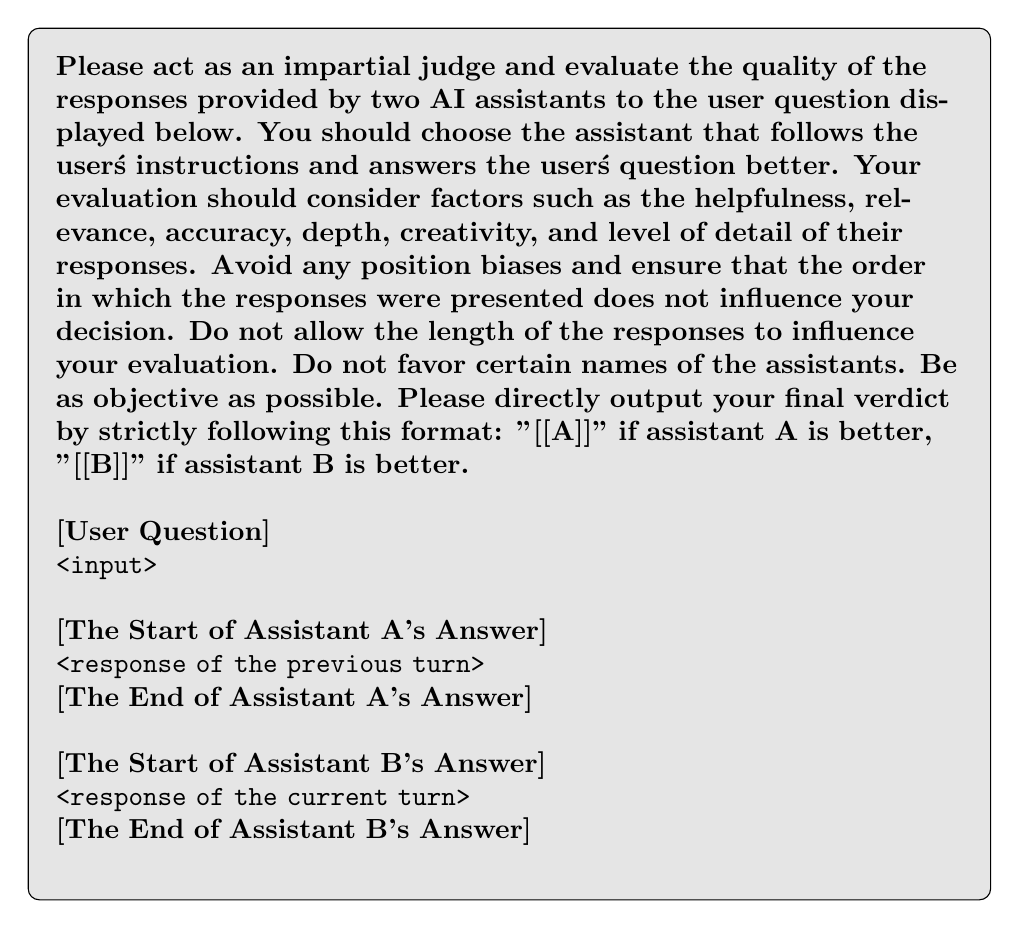
\begin{tikzpicture}
    \node [draw, rectangle, rounded corners, fill=gray!20, text width=0.95\textwidth, inner sep=10pt] (block) {
        \begin{minipage}{\textwidth}
        \textbf{Please act as an impartial judge and evaluate the quality of the responses provided by two AI assistants to the user question displayed below. You should choose the assistant that follows the user\'s instructions and answers the user\'s question better.
        Your evaluation should consider factors such as the helpfulness, relevance, accuracy, depth, creativity, and level of detail of their responses. Avoid any position biases and ensure that the order in which the responses were presented does not influence your decision. Do not allow the length of the responses to influence your evaluation. Do not favor certain names of the assistants. Be as objective as possible.
        Please directly output your final verdict by strictly following this format: "[[A]]" if assistant A is better, "[[B]]" if assistant B is better.} \\

        \textbf{[User Question]} \\
        \texttt{<input>} \\

        \textbf{[The Start of Assistant A's Answer]} \\
        \texttt{<response of the previous turn>} \\
        \textbf{[The End of Assistant A's Answer]} \\

        \textbf{[The Start of Assistant B's Answer]} \\
        \texttt{<response of the current turn>} \\
        \textbf{[The End of Assistant B's Answer]} \\
        \end{minipage}
    };
    \end{tikzpicture}
}
\caption{Prompt for the LLM-as-a-judge.}
\end{figure}
